\section{Backend Code Structure (Rust Actix-Web)}

\subsection{ภาพรวมสถาปัตยกรรม}

Backend ใช้ภาษา \textbf{Rust} ร่วมกับ Framework \textbf{Actix-Web} ซึ่งเป็น Web Framework ที่มีประสิทธิภาพสูงสุดตัวหนึ่ง 
โครงสร้างโค้ดออกแบบตามหลัก \textbf{Clean Architecture / Layered Architecture} 
แบ่ง Layer ชัดเจนเพื่อให้ง่ายต่อการทดสอบ (Testability) และการบำรุงรักษา (Maintainability)

\begin{figure}[h]
    \centering
    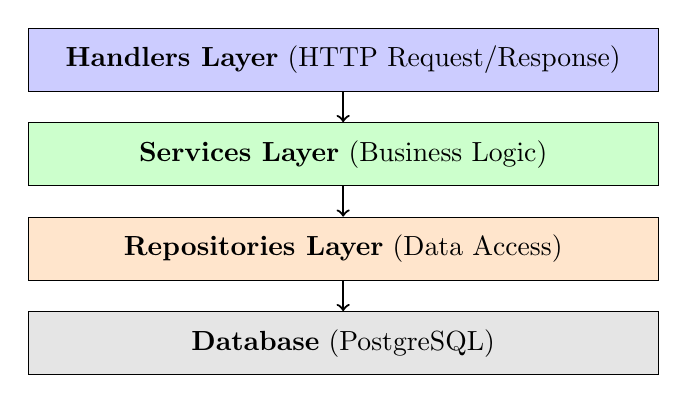
\begin{tikzpicture}[node distance=1.2cm]
        \tikzstyle{layer} = [rectangle, draw, minimum width=8cm, minimum height=0.8cm, align=center]
        
        \node (handlers) [layer, fill=blue!20] {\textbf{Handlers Layer} (HTTP Request/Response)};
        \node (services) [layer, fill=green!20, below of=handlers] {\textbf{Services Layer} (Business Logic)};
        \node (repos) [layer, fill=orange!20, below of=services] {\textbf{Repositories Layer} (Data Access)};
        \node (db) [layer, fill=gray!20, below of=repos] {\textbf{Database} (PostgreSQL)};
        
        \draw[->, thick] (handlers) -- (services);
        \draw[->, thick] (services) -- (repos);
        \draw[->, thick] (repos) -- (db);
    \end{tikzpicture}
    \caption{Layered Architecture ของระบบ Backend}
    \label{fig:layered_arch}
\end{figure}

\clearpage

\subsection{โครงสร้างไดเรกทอรี (Directory Structure)}

\dirtree{%
.1 project-root/.
.2 Cargo.lock.
.2 Cargo.toml.
.2 .env.
.2 .env.example.
.2 tests/.
.3 integration/.
.4 ....
.2 migrations/.
.3 <timestamp>\_create\_tables.sql.
.2 src/.
.3 main.rs \textit{--- Application entry point}.
.3 lib.rs \textit{--- Re-exports for modules}.
.3 routes.rs \textit{--- Route configuration}.
.3 config/.
.4 mod.rs.
.4 settings.rs \textit{--- AppConfig, DatabaseConfig, JWTConfig}.
.3 db/.
.4 mod.rs.
.4 connection.rs \textit{--- PgPool setup}.
.3 models/.
.4 mod.rs.
.4 user.rs.
.4 folder.rs.
.4 image.rs.
.4 job.rs.
.4 analysis\_result.rs.
.3 dto/.
.4 mod.rs.
.4 auth\_dto.rs.
.4 folder\_dto.rs.
.4 image\_dto.rs.
.4 job\_dto.rs.
.4 analysis\_dto.rs.
.3 domain/.
.4 mod.rs.
.4 error.rs \textit{--- AppError, ApiResponse wrapper}.
.3 handlers/.
.4 mod.rs.
.4 auth\_handlers.rs.
.4 folder\_handlers.rs.
.4 image\_handlers.rs.
.4 job\_handlers.rs.
.4 analysis\_handlers.rs.
.3 middleware/.
.4 mod.rs.
.4 auth\_middleware.rs.
.4 error\_middleware.rs.
.3 repositories/.
.4 mod.rs.
.4 user\_repository.rs.
.4 folder\_repository.rs.
.4 image\_repository.rs.
.4 job\_repository.rs.
.4 analysis\_repository.rs.
.3 services/.
.4 mod.rs.
.4 auth\_service.rs.
.4 token\_service.rs.
.4 folder\_service.rs.
.4 image\_service.rs.
.4 storage\_service.rs.
.4 job\_service.rs.
.4 ai\_inference\_service.rs.
.3 workers/ \textit{--- Background Job Processing}.
.4 mod.rs.
.4 analysis\_worker.rs \textit{--- AI Analysis Job Runner}.
.4 job\_scheduler.rs \textit{--- Job Queue Management}.
.3 utils/.
.4 mod.rs.
.4 file\_utils.rs.
.4 validation.rs.
.4 response.rs \textit{--- ApiResponse helpers}.
}

\clearpage

\subsection{คำอธิบายแต่ละ Module}

\subsubsection{config/ - การตั้งค่าระบบ}
จัดการ Environment Variables และการตั้งค่าต่างๆ ของระบบ

\begin{table}[h!]
    \centering
    \begin{tabular}{|l|p{9cm}|}
        \hline
        \textbf{ไฟล์} & \textbf{หน้าที่} \\
        \hline
        settings.rs & โครงสร้างสำหรับเก็บค่า Config เช่น Database URL, JWT Secret, Server Port, CORS Settings \\
        \hline
    \end{tabular}
\end{table}

\subsubsection{db/ - การเชื่อมต่อฐานข้อมูล}
จัดการ Connection Pool สำหรับฐานข้อมูล PostgreSQL

\begin{table}[h!]
    \centering
    \begin{tabular}{|l|p{9cm}|}
        \hline
        \textbf{ไฟล์} & \textbf{หน้าที่} \\
        \hline
        connection.rs & สร้างและจัดการ PgPool (Connection Pooling) ด้วย SQLx \\
        \hline
    \end{tabular}
\end{table}

\subsubsection{models/ - Database Entities}
กำหนดโครงสร้างข้อมูลที่ตรงกับตารางในฐานข้อมูล (ORM Mapping)

\begin{table}[h!]
    \centering
    \begin{tabular}{|l|p{9cm}|}
        \hline
        \textbf{ไฟล์} & \textbf{หน้าที่} \\
        \hline
        user.rs & Struct สำหรับตาราง Users \\
        \hline
        folder.rs & Struct สำหรับตาราง Folders \\
        \hline
        image.rs & Struct สำหรับตาราง Images \\
        \hline
        job.rs & Struct สำหรับตาราง Jobs \\
        \hline
        analysis\_result.rs & Struct สำหรับตาราง Analysis\_Results \\
        \hline
    \end{tabular}
\end{table}

\subsubsection{dto/ - Data Transfer Objects}
โครงสร้างข้อมูลสำหรับ Request/Response แยกจาก Database Models

\begin{table}[h!]
    \centering
    \begin{tabular}{|l|p{9cm}|}
        \hline
        \textbf{ไฟล์} & \textbf{หน้าที่} \\
        \hline
        auth\_dto.rs & LoginRequest, RegisterRequest, TokenResponse \\
        \hline
        folder\_dto.rs & CreateFolderRequest, FolderResponse, UpdateFolderRequest \\
        \hline
        image\_dto.rs & ImageUploadResponse, ImageDetailResponse \\
        \hline
        job\_dto.rs & JobStatusResponse, CreateJobRequest \\
        \hline
        analysis\_dto.rs & AnalysisResultResponse, AnalysisSummary \\
        \hline
    \end{tabular}
\end{table}

\clearpage

\subsubsection{domain/ - Business Logic Core}
กฎเกณฑ์ทางธุรกิจและการจัดการ Error กลาง

\begin{table}[h!]
    \centering
    \begin{tabular}{|l|p{9cm}|}
        \hline
        \textbf{ไฟล์} & \textbf{หน้าที่} \\
        \hline
        error.rs & กำหนด AppError enum และ implement ResponseError trait สำหรับแปลง Error เป็น HTTP Response \\
        \hline
    \end{tabular}
\end{table}

\subsubsection{handlers/ - HTTP Handlers}
รับ HTTP Request และส่ง Response กลับไปยัง Client (Controller Layer)

\begin{table}[h!]
    \centering
    \begin{tabular}{|l|p{9cm}|}
        \hline
        \textbf{ไฟล์} & \textbf{หน้าที่} \\
        \hline
        auth\_handlers.rs & register(), login(), logout() \\
        \hline
        folder\_handlers.rs & list\_folders(), create\_folder(), update\_folder(), delete\_folder() \\
        \hline
        image\_handlers.rs & list\_images(), upload\_image(), get\_image(), delete\_image() \\
        \hline
        job\_handlers.rs & get\_job\_status() \\
        \hline
        analysis\_handlers.rs & analyze\_image(), get\_result(), get\_history() \\
        \hline
    \end{tabular}
\end{table}

\subsubsection{middleware/ - Middleware Layer}
ประมวลผล Request/Response ก่อนถึง Handler

\begin{table}[h!]
    \centering
    \begin{tabular}{|l|p{9cm}|}
        \hline
        \textbf{ไฟล์} & \textbf{หน้าที่} \\
        \hline
        auth\_middleware.rs & ตรวจสอบ JWT Token และแนบข้อมูล User ไปกับ Request \\
        \hline
        error\_middleware.rs & จัดการ Error แบบ Global และแปลงเป็น JSON Response มาตรฐาน \\
        \hline
    \end{tabular}
\end{table}

\subsubsection{repositories/ - Data Access Layer}
ดำเนินการ CRUD กับฐานข้อมูลโดยตรง

\begin{table}[h!]
    \centering
    \begin{tabular}{|l|p{9cm}|}
        \hline
        \textbf{ไฟล์} & \textbf{หน้าที่} \\
        \hline
        user\_repository.rs & find\_by\_id(), find\_by\_username(), create(), update() \\
        \hline
        folder\_repository.rs & find\_all\_by\_user(), create(), update(), delete() \\
        \hline
        image\_repository.rs & find\_by\_folder(), create(), delete(), count\_by\_folder() \\
        \hline
        job\_repository.rs & create(), update\_status(), find\_by\_image() \\
        \hline
        analysis\_repository.rs & create(), find\_by\_job(), find\_history\_by\_image() \\
        \hline
    \end{tabular}
\end{table}

\clearpage

\subsubsection{services/ - Business Logic Layer}
รวม Business Logic และประสานงานระหว่าง Repositories

\begin{table}[h!]
    \centering
    \begin{tabular}{|l|p{9cm}|}
        \hline
        \textbf{ไฟล์} & \textbf{หน้าที่} \\
        \hline
        auth\_service.rs & ตรวจสอบข้อมูลผู้ใช้, เข้ารหัสรหัสผ่าน, จัดการ Login/Logout \\
        \hline
        token\_service.rs & สร้างและ Verify JWT/PASETO Tokens \\
        \hline
        folder\_service.rs & Logic การจัดการโฟลเดอร์ (ตรวจสอบสิทธิ์, Cascade Delete) \\
        \hline
        image\_service.rs & จัดการอัปโหลดภาพ, แยก Metadata, ย่อขนาด Thumbnail \\
        \hline
        storage\_service.rs & จัดการไฟล์บน Disk หรือ Object Storage (S3-compatible) \\
        \hline
        job\_service.rs & สร้าง Job, อัปเดตสถานะ, ติดตาม Progress \\
        \hline
        ai\_inference\_service.rs & ส่งภาพไป AI Model Service และรับผลลัพธ์กลับมา \\
        \hline
    \end{tabular}
\end{table}

\subsubsection{workers/ - Background Job Processing}
จัดการงานที่ประมวลผลแบบ Asynchronous (Background Tasks) โดยเฉพาะการวิเคราะห์ภาพด้วย AI ที่ใช้เวลานาน

\begin{table}[h!]
    \centering
    \begin{tabular}{|l|p{9cm}|}
        \hline
        \textbf{ไฟล์} & \textbf{หน้าที่} \\
        \hline
        analysis\_worker.rs & รับ Job จาก Queue, ส่งภาพไป AI Service, บันทึกผลลัพธ์, อัปเดตสถานะ Job \\
        \hline
        job\_scheduler.rs & จัดการ Job Queue, กำหนด Retry Policy, จัดลำดับความสำคัญของ Jobs \\
        \hline
    \end{tabular}
\end{table}

\textbf{Flow การทำงาน:}
\begin{enumerate}
    \item Client เรียก \texttt{POST /images/\{id\}/analyze} → สร้าง Job (status: pending) → ตอบ 202 Accepted
    \item \texttt{job\_scheduler.rs} ดึง Job ที่ pending มาประมวลผล
    \item \texttt{analysis\_worker.rs} เรียก AI Service และบันทึกผล
    \item Client ใช้ \texttt{GET /jobs/\{id\}} เพื่อ Polling ตรวจสอบสถานะ
\end{enumerate}

\subsubsection{utils/ - Utility Functions}
ฟังก์ชันช่วยเหลือทั่วไป

\begin{table}[h!]
    \centering
    \begin{tabular}{|l|p{9cm}|}
        \hline
        \textbf{ไฟล์} & \textbf{หน้าที่} \\
        \hline
        file\_utils.rs & สร้างชื่อไฟล์ UUID, ตรวจสอบ MIME Type, คำนวณ Hash \\
        \hline
        validation.rs & Validation helpers สำหรับ Input (ใช้ร่วมกับ validator crate) \\
        \hline
        response.rs & Helper สำหรับสร้าง API Response มาตรฐาน \\
        \hline
    \end{tabular}
\end{table}

\subsubsection{routes.rs - Route Configuration}
รวมการตั้งค่า Routes ทั้งหมดไว้ที่เดียว

\begin{verbatim}
pub fn configure_routes(cfg: &mut web::ServiceConfig) {
    cfg.service(
        web::scope("/api/v1")
            .configure(auth_routes)
            .configure(folder_routes)
            .configure(image_routes)
            .configure(job_routes)
            .configure(analysis_routes)
    );
}
\end{verbatim}

\clearpage

\subsection{Dependencies (Cargo.toml)}

การเลือก Dependencies สำหรับโปรเจกต์นี้พิจารณาจาก 3 ปัจจัยหลัก: \textbf{ความปลอดภัย (Security)}, \textbf{ประสิทธิภาพ (Performance)}, และ \textbf{ความน่าเชื่อถือ (Reliability)} โดยอ้างอิงจากมาตรฐานอุตสาหกรรมและ Best Practices จากชุมชน Rust

\subsubsection{Core Framework}

\paragraph{actix-web}
Web Framework อันดับ 1 ของ Rust ใน TechEmpower Benchmarks ด้วยสถาปัตยกรรม Actor Model ที่สามารถรองรับ Request ได้มากกว่า 500,000 req/sec บน Hardware ทั่วไป มี Memory Safety จาก Rust Compiler และไม่มี Runtime Overhead จาก Garbage Collection

\paragraph{tokio}
Async Runtime มาตรฐานของ Rust Ecosystem ใช้โดยบริษัทระดับโลก เช่น Discord, Cloudflare, และ AWS ให้ความสามารถ Concurrent I/O แบบ Non-blocking ด้วย Work-stealing Scheduler ที่มีประสิทธิภาพสูง

\subsubsection{Database \& ORM}

\paragraph{sqlx}
Async SQL Toolkit ที่มีความสามารถพิเศษคือ \textbf{Compile-time Query Verification} ซึ่งจะตรวจสอบ SQL Query กับ Database Schema ตั้งแต่ตอน Compile ทำให้ไม่มีโอกาสเกิด SQL Syntax Error หรือ Type Mismatch ใน Production และป้องกัน SQL Injection โดยอัตโนมัติผ่าน Prepared Statements

\subsubsection{Authentication \& Security}

\paragraph{argon2}
Password Hashing Algorithm ที่ชนะการแข่งขัน Password Hashing Competition (PHC) ในปี 2015 และได้รับการแนะนำจาก \textbf{OWASP (Open Web Application Security Project)} ให้เป็นมาตรฐานสำหรับการเข้ารหัสรหัสผ่าน มีความต้านทานต่อ GPU Cracking และ Side-channel Attacks

\paragraph{rusty\_paseto}
PASETO (Platform-Agnostic Security Tokens) เป็นเทคโนโลยีทดแทน JWT ที่ออกแบบมาเพื่อแก้ไขจุดอ่อนด้านความปลอดภัยของ JWT:
\begin{itemize}
    \item ไม่มี Algorithm Confusion Attack (ไม่ต้องระบุ Algorithm ใน Header)
    \item บังคับใช้ Encryption ที่ปลอดภัย (XChaCha20-Poly1305 หรือ Ed25519)
    \item ไม่สามารถใช้ Algorithm ``none'' หรือ Algorithm ที่อ่อนแอได้
\end{itemize}

\paragraph{secrecy}
Library สำหรับจัดการข้อมูลลับ (Secrets) โดยป้องกันไม่ให้ข้อมูลสำคัญ เช่น Password หรือ API Keys หลุดไปใน Log Files หรือ Error Messages ผ่านการ Implement \texttt{Debug} และ \texttt{Display} traits ที่ซ่อนค่าจริง

\paragraph{rustls}
TLS Library แบบ Pure Rust ที่ไม่พึ่งพา OpenSSL ซึ่งมีประวัติช่องโหว่ร้ายแรง (เช่น Heartbleed) Rustls ผ่านการ Audit จาก Cure53 และ Trail of Bits มีความปลอดภัยจาก Memory Safety ของ Rust

\subsubsection{Rate Limiting \& Protection}

\paragraph{actix-governor}
Rate Limiting Middleware ที่ใช้ Algorithm Generic Cell Rate Algorithm (GCRA) ป้องกัน:
\begin{itemize}
    \item \textbf{DDoS Attack:} จำกัดจำนวน Request ต่อ IP
    \item \textbf{Brute Force Attack:} ป้องกันการเดา Password
    \item \textbf{API Abuse:} ควบคุมการใช้งาน API ไม่ให้เกินกำหนด
\end{itemize}

\subsubsection{Validation \& Serialization}

\paragraph{validator}
Input Validation Library ที่ใช้ Derive Macros ทำให้สามารถกำหนด Validation Rules ผ่าน Attributes บน Struct Fields ได้โดยตรง ลดโอกาสที่จะลืม Validate Input และป้องกัน Injection Attacks

\paragraph{serde / serde\_json}
De-facto Standard สำหรับ Serialization/Deserialization ใน Rust Ecosystem ใช้โดยเกือบทุก Library ที่ต้องจัดการกับข้อมูล JSON มี Zero-copy Deserialization สำหรับ Performance และ Type Safety สูง

\subsubsection{Performance Optimization}

\paragraph{jemallocator}
Memory Allocator จาก FreeBSD ที่ Facebook ใช้ใน Production เหมาะกับ Multi-threaded Applications ลด Memory Fragmentation และเพิ่ม Performance ได้ 10-30\% เมื่อเทียบกับ System Allocator

\paragraph{compress-zstd}
Zstandard Compression Algorithm พัฒนาโดย Facebook ให้ Compression Ratio ใกล้เคียง gzip แต่เร็วกว่า 3-5 เท่า เหมาะสำหรับ Compress HTTP Response เพื่อลด Bandwidth

\subsubsection{Observability}

\paragraph{tracing}
Structured Logging และ Distributed Tracing Library มาตรฐานของ Rust รองรับ OpenTelemetry Protocol สำหรับส่ง Traces ไปยัง Jaeger, Zipkin หรือ Cloud Services ทำให้สามารถ Debug และ Monitor ระบบ Production ได้อย่างมีประสิทธิภาพ

\subsubsection{Identifiers}

\paragraph{uuid}
Library สำหรับสร้างและจัดการ UUID (Universally Unique Identifier) เวอร์ชัน 4 ซึ่งสร้างจาก Cryptographically Secure Random Number Generator (CSPRNG) ใช้เป็น Primary Key และ Session ID เพื่อป้องกัน ID Enumeration Attack

\subsubsection{Security Audit Tools}

\paragraph{cargo-audit}
เครื่องมือตรวจสอบ Dependencies กับฐานข้อมูล RustSec Advisory Database ซึ่งรวบรวมช่องโหว่ความปลอดภัยของ Crates ทั้งหมด ควรรันใน CI/CD Pipeline ทุกครั้งก่อน Deploy

\paragraph{cargo-deny}
เครื่องมือตรวจสอบ License Compliance และ Security Policy ป้องกันการใช้ Crates ที่มี License ไม่เหมาะสม หรือมีช่องโหว่ที่ยังไม่ได้แก้ไข

\clearpage

\subsection{Release Profile Optimization}

การตั้งค่า Release Build เพื่อประสิทธิภาพสูงสุดและขนาดไฟล์เล็ก:

\begin{verbatim}
[profile.release]
opt-level = 3       # Optimization สูงสุด
lto = true          # Link Time Optimization
codegen-units = 1   # Single codegen unit (optimize ดีที่สุด)
panic = "abort"     # ตัด panic unwinding code
strip = true        # ลบ debug symbols
\end{verbatim}

\begin{table}[h!]
    \centering
    \begin{tabular}{|l|p{9cm}|}
        \hline
        \textbf{Option} & \textbf{ผลลัพธ์} \\
        \hline
        \texttt{opt-level = 3} & จูนความเร็วสูงสุด (Runtime Performance) \\
        \hline
        \texttt{lto = true} & Link Time Optimization ทำให้ Binary เล็กลงและเร็วขึ้น \\
        \hline
        \texttt{codegen-units = 1} & Compile ช้าขึ้นแต่ Optimize Code ได้ดีที่สุด \\
        \hline
        \texttt{panic = "abort"} & ลดขนาดไฟล์โดยตัด Stack Trace Handling ออก \\
        \hline
        \texttt{strip = true} & ลบ Debug Symbols (ลดขนาด Binary มหาศาล) \\
        \hline
    \end{tabular}
    \caption{Release Profile Options}
    \label{tab:release_profile}
\end{table}

\subsection{ตัวอย่าง Cargo.toml}

\begin{verbatim}
[package]
name = "cell-analysis-backend"
version = "0.1.0"
edition = "2021"

[dependencies]
actix-web = "4"
actix-governor = "0.5"
actix-cors = "0.7"
actix-web-httpauth = "0.8"
tokio = { version = "1", features = ["full"] }
sqlx = { version = "0.7", features = ["runtime-tokio", 
         "postgres", "uuid", "chrono", "json"] }
serde = { version = "1", features = ["derive"] }
serde_json = "1"
uuid = { version = "1", features = ["v4", "serde"] }
validator = { version = "0.16", features = ["derive"] }
argon2 = "0.5"
secrecy = { version = "0.8", features = ["serde"] }
rusty_paseto = "0.6"
rustls = "0.22"
tracing = "0.1"
tracing-subscriber = "0.3"
chrono = { version = "0.4", features = ["serde"] }
thiserror = "1"

[target.'cfg(not(target_env = "msvc"))'.dependencies]
jemallocator = "0.5"

[profile.release]
opt-level = 3
lto = true
codegen-units = 1
panic = "abort"
strip = true
\end{verbatim}

\clearpage

\subsection{Data Flow Diagram}

\begin{figure}[h]
    \centering
    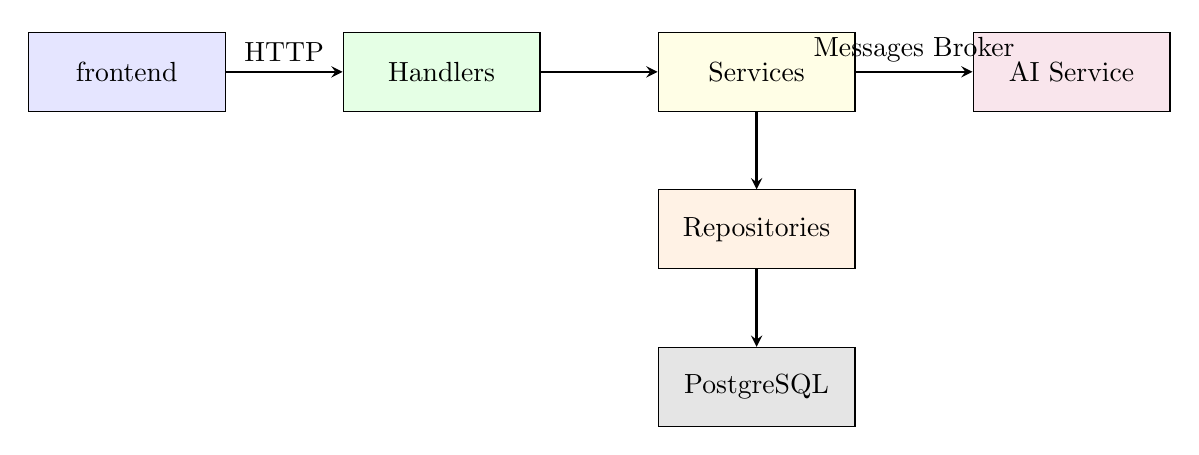
\begin{tikzpicture}[node distance=2cm]
        \tikzstyle{process} = [rectangle, draw, minimum width=2.5cm, minimum height=1cm, align=center]
        \tikzstyle{arrow} = [thick,->,>=stealth]
        
        \node (client) [process, fill=blue!10] {frontend};
        \node (handler) [process, fill=green!10, right of=client, xshift=2cm] {Handlers};
        \node (service) [process, fill=yellow!10, right of=handler, xshift=2cm] {Services};
        \node (repo) [process, fill=orange!10, below of=service] {Repositories};
        \node (db) [process, fill=gray!20, below of=repo] {PostgreSQL};
        \node (ai) [process, fill=purple!10, right of=service, xshift=2cm] {AI Service};
        
        \draw [arrow] (client) -- node[above] {HTTP} (handler);
        \draw [arrow] (handler) -- (service);
        \draw [arrow] (service) -- (repo);
        \draw [arrow] (repo) -- (db);
        \draw [arrow] (service) -- node[above] {Messages Broker} (ai);
    \end{tikzpicture}
    \caption{Data Flow ระหว่าง Components}
    \label{fig:data_flow}
\end{figure}

\subsection{ข้อดีของโครงสร้างนี้}

\begin{enumerate}
    \item \textbf{Separation of Concerns:} แต่ละ Layer มีหน้าที่ชัดเจน ไม่ปนกัน
    \item \textbf{Testability:} สามารถ Unit Test แต่ละ Layer แยกกันได้ง่าย โดยใช้ Mock
    \item \textbf{Maintainability:} เมื่อต้องแก้ไข Business Logic ก็แก้เฉพาะ Services Layer
    \item \textbf{Scalability:} สามารถแยก Services ออกเป็น Microservices ได้ในอนาคต
    \item \textbf{Security:} แยกการจัดการ Authentication/Authorization ไว้ใน Middleware
    \item \textbf{Performance:} Rust + Actix-Web ให้ประสิทธิภาพสูงมาก พร้อม Memory Safety
\end{enumerate}

\subsection{Standard}
